% -*-coding: utf-8;-*-
%\chapter{Нейросетевое управление в нестационарных условиях}

Во большинстве случаев система управления проектируется исходя из
предположения о постоянстве её параметров, однако в реальном мире нет
ничего неизменного.  Элементы системы управления со временем
изнашиваются, условия внешней среды меняются, в процессе
функционирования возможны случайные деструктивные воздействия,
меняющие характеристики элементов системы, например, аварии.  Эти
процессы иногда можно предвидеть, но всегда трудно точно описать,
поскольку они носят вероятностный характер.

Фактор износа элементов системы можно учесть, расчитав срок их
эксплуатации и проводя превентивную замену давно работающего элемента
на новый с номинальными характеристиками.  Вариации условий внешней
среды можно заложить в исходную модель в качестве возмущающих
воздействий или просто на модели убедиться в сохранении устойчивости и
качества функционирования системы управления во всем диапазоне
возможных изменений внешних условий.  Эти решения дают
удовлетворительный результат, однако их отличает то, что они
неоптимальны, а значит, приводят к экономическим потерям: замене по
регламенту ещё вполне исправных элементов, неоптимальной работе
контура управления в течение длительных периодов отличия внешних
условий от расчетных.

Случайные воздействия на элементы системы автоматического управления
совершенно непредсказуемы и по вероятности их возникновения и по
производимому эффекту.  Случаи катастофических изменений, как правило,
легко отслеживаются и исправляются заменой вышедших из строя
элементов.  Однако, небольшие изменения вызывают малозаметные
отклонения в штатном функционировании системы, которые могут привести
к серьезным последствиям черех некоторое время: повышенному износу,
браку, сбоям в других связанных системах управления.

Вышеперечисленные факторы однозначно свидетельствуют о важности
развития методов автоматического управления, адаптированным к
нестационарному поведению объекта.  Наиболее целесообразным
представляется рассмотреть случай ступенчатого изменения свойств
объекта.  Рассмотрим нейросетевые методы управления нестационарным
объектом.

\section{Метод постоянной адаптации}

Для решения предложенной задачи достаточно распространенным является
подход с постоянной адаптацией нейросетевого регулятора \cite{XXX}.  В
этом случае нейронная сеть будет подстраиваться к изменениям
динамических характеристик объекта.  Данный подход можно реализовать в
рамках алгоритмов настройки нейросетевого регулятора, использующих
прямую или косвенную нейросетевую инверсию объекта управления.
Сделаем это, развивая метод косвенного адаптивного управления
(indirect adaptive control) на случай нестационарного объекта
\cite{XXX}.

В рамках этой методики настройка нейросетевого регулятора производится
с помощью предварительно обученной нейронной сети идентификатора
(см. \ref{XXX}), функционирующей подобно объекту управления.  В
стационарных условиях нейросетевая идентификация может быть проведена
один раз.  Однако при изменении динамических свойств объекта
управления требуется адаптация как нейросетевого регулятора, так и
нейронной сети идентификатора.  При постоянной активности алгоритма
адаптации обе нейронных сети непрерывно находятся в состоянии
настройки.  На \figref{fig:permanent_adoption_loop} приводится схема
системы управления с алгоритмом постоянной адаптации.

\begin{figure}[h]
\centering
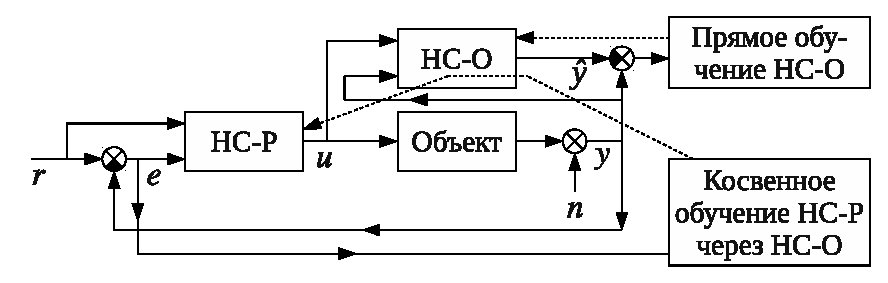
\includegraphics{permanent_adoption_rus}
\caption{Контур управления со схемой постоянной адаптации.}
\label{fig:permanent_adoption_loop}
\end{figure}

Внешними входными сигналами системы управления являются уставка $r$ и
аддитивная помеха $n$ наблюдаемого выхода объекта.  Нейросетевой
регулятор (НС--Р) оказывает на объект управления воздействие $u$ с
целью минимизировать ошибку управления $e=r-y$.  Параллельно объекту
включена нейронная сеть идентификатора (НС--О), которая по управляющему
воздействию регулятора $u$ и предыдущим наблюдениям выхода объекта $y$
предсказывает выход объекта $\hat{y}$ в следующий момент времени.

Одновременно включены два алгоритма настройки нейронных сетей: прямое
обучение нейросетевого идентификатора на основе ошибки идентификации
$d=y-\hat{y}$ и косвенное обучение нейросетевого регулятора путем
обратного распространения ошибки управления $e$ через НС--О к НС--Р
(см. \ref{XXX}).  Направления обратного распространения ошибки
показаны на схеме пунктирными линиями.

В схеме постоянной адаптации используются нейронные сети прямого
распространения.  Архитектура нейронных сетей регулятора и
идентификатора показана на \figref{fig:nonst_nn_schema}.  Для лучшего
моделирования динамики объекта управления на вход НС--О подаются
сигналы $u$ и $y$ нескольких прошлых моментов времени $D_u$ и $D_y$
соответственно (\figref{fig:nonst_nn_schema}а).  Нейросетевой
регулятор получает на вход не только значение ошибки управления, но и
уставку (\figref{fig:nonst_nn_schema}б).  Это обеспечивает динамику
регулирования при отсутствии обратных связей в нейросети.

\begin{figure}[h]
\centering
\begin{tabular}{cc}
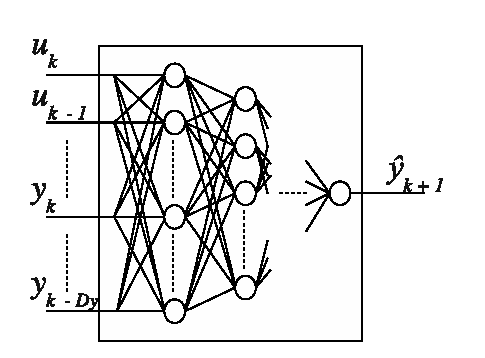
\includegraphics{nonst_nnp_schema} & 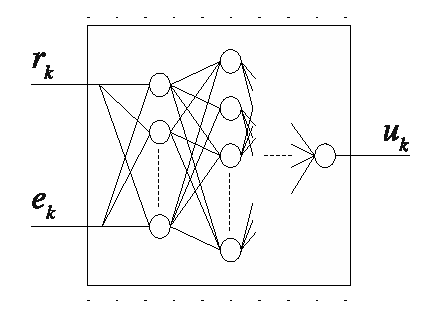
\includegraphics{nonst_nnc_schema} \\
а) & б)\\
\end{tabular}
\caption{Архитектура нейронных сетей модели объекта (а) и регулятора (б).}
\label{fig:nonst_nn_schema}
\end{figure}

Следует особо отметить три важных момента, касающихся изложенной схемы
обучения.  Во-первых, в процессе обратного распространения ошибки
управления через нейросеть идентификатора поправки весовых
коэффициентов рассчитываются, но не применяются, поскольку задача
минимизации ошибки управления возлагается на нейронную сеть
регулятора, чьи весовые коэффициенты изменяются с этой целью.
Во-вторых, процесс обучения нейросети идентификатора проходит
независимо от обучения регулятора, то есть, поправки весовых
коэффициентов рассчитываются независимо и не влияют друг на друга.  В
отличие от обучения НС--О вне контура управления (см. \ref{XXX}), в
данном случае обучение происходит в контуре в реальном времени и без
контрольной выборки.  В третьих, рассчитанные изменения весовых
коэффициентов нейронных сетей суммируются на протяжении нескольких
тактов работы дискретной системы управления и применяются (изменяют
нейронную сеть) с некоторой периодичностью подобно пакетному методу.
Это позволяет отстроиться от незакономерных атомарных изменений
весовых коэффициентов.  Пакетное обучение нейронной сети вне контура
управления обычно применяется для ускорения процесса обучения, но в
данном случае этот подход позволяет стабилизировать контур управления,
поскольку случайные некорректные изменения НС--О могут привести к
некорректному изменению НС--Р, а это может вывести контур управления из
устойчивости.

\section{Метод адаптации по обнаружению разладки}

Другим способом подстройки нейросетевого регулятора является
модернизированный подход, который в стационарных условиях не
предполагает изменения нейронных сетей, однако при этом функционирует
блок обнаружения изменения свойств объекта управления ---
разладки~(\figref{fig:steady_state_loop}).  После обнаружения разладки
осуществляется сбор необходимых данных и производится обучение
нейронной сети идентификатора НС--О вне контура управления.  По
окончании обучения нейросетевого идентификатора он включается в
активированную схему адаптации нейросетевого регулятора
НС--Р~(\figref{fig:modified_adoption_loop}) аналогично схеме синтеза
оптимального нейросетевого регулятора в стационарном случае
(см.~\cite{XXX}).  Следует отметить, что в предложенной схеме
используются нейронные сети полностью аналогичной архитектуры, что и в
методе с постоянной адаптацией~(\figref{fig:nonst_nn_schema}).

\begin{figure}[h]
\centering
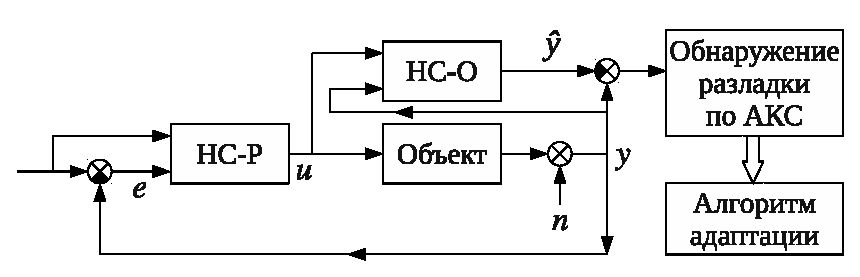
\includegraphics{steady_state_rus}
\caption{Контур управления в стационарном режиме.}
\label{fig:steady_state_loop}
\end{figure}

\begin{figure}[h]
\centering
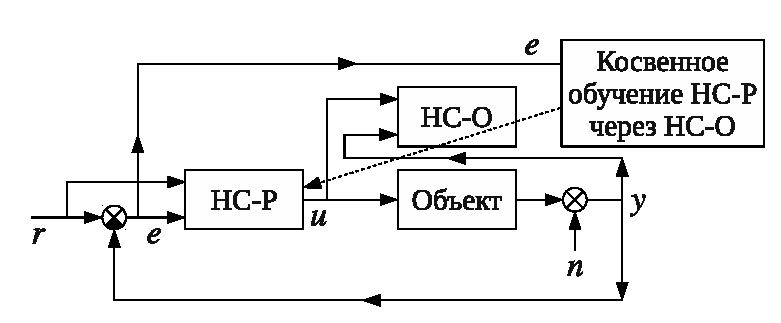
\includegraphics{modified_adoption_rus}
\caption{Контур управления в режиме адаптации к разладке.}
\label{fig:modified_adoption_loop}
\end{figure}

Для того чтобы эта схема работала в нестационарных условиях,
необходимо надежно определять момент изменения параметров объекта
управления и сообразно подстраивать его нейросетевую модель.

Задача определения разладки решается с помощью алгоритма кумулятивных
сумм (АКС), причем для надежности обнаружения разладки берется парное
срабатывание в пределах расчетного среднего времени запаздывания.
Подстройка нейросетевой модели объекта управления осуществляется вне
контура управления способом, изложенным в п.~\ref{XXX}.  Для обучения
нейронной сети в этом случае необходимо подготовить обучающие данные в
объеме, достаточном для качественного предсказания поведения объекта и
обучения нейросетевого регулятора.  Поскольку предполагается
автоматический характер процедуры адаптации регулятора, необходимо
сформулировать обоснованный алгоритм сбора данных.  Рассмотрим решение
этих задач более подробно.

\subsection{Настройка АКС}

% Описать АКС с необходимой подробностью

Для обеспечения необходимых свойств алгоритма обнаружения разладки
необходима соответствующая настройка АКС. Как известно, главным
управляемым параметром классического АКС является решающая граница
(порог) $H$ ({\em threshold}), а основными характеристиками ---
среднее время запаздывания $T_{ad}$ ({\em time of average alarm's
  delay}) и среднее время между ложными тревогами $T_{fa}$ ({\em time
  between false alarms}).  Применительно к рассматриваемой задаче они
определяют время, в течение которого будут продолжаться потери,
возникающие в результате изменения параметров объекта управления.

Для настройки АКС нужно задать значение контролируемого параметра в
исходном состоянии (до разладки), ожидаемое значение этого же
параметра при разладке (номинальная разладка), а также выбрать порог
$H>0$, обеспечивающий желаемые значения $T_{ad}$ и
$T_{fa}$. Предварительные эксперименты показали, что в качестве
параметра, по которому хорошо определяется изменение параметров
объекта управления, следует использовать дисперсию ошибки
идентификации $d=y-\hat{y}$.  За исходное значение следует принять
дисперсию, определенную для стационарного режима $\sigma^2_0$, а за
номинальную разладку --- ее увеличение в заданное число раз (например,
$K=2$): $\sigma^2_1=K\sigma^2_0$.

Для определения разладки по дисперсии случайного процесса с нормальным
распределением слагаемые в уравнении изображающей точки АКС
вычисляются по формуле:
\begin{equation}
  z_i=-\frac{1}{2}\ln\frac{\sigma^2_1}{\sigma^2_0}-\frac{1}{2}
  \left(\frac{1}{\sigma^2_1}-\frac{1}{\sigma^2_0}\right)d_i^2
\end{equation}

Само уравнение изображающей точки в классическом АКС при выполнении
элементарной проверочной процедуры имеет вид:
\begin{equation}
  S_i=\left\{
  \begin{array}{ll}
    0, & i=0\\
    \max\left(0; S_{i-1}+z_i\right), & i>0\\
  \end{array}\right.
\end{equation}

Критерием разладки является
\begin{equation}
  S_i>H
\end{equation}

\noindent то есть, достижение изображающей точкой $S_i$ решающей
границы $H$.  В этом случае разладка считается обнаруженной,
элементарная проверочная процедура заканчивается и при необходимости
начинается следующая проверочная процедура.  Чем выше порог, тем
больше задержка между фактическим изменением параметров случайного
процесса и моментом обнаружения разладки.  С другой стороны, малое
значение порога приводит к росту случаев ложного срабатывания в силу
случайности процесса.

Настройка АКС осуществляется путем выбора $H$ исходя из некоторого
компромисса между значениями $T_{ad}$ и $T_{fa}$.  С целью более
надежной диагностики разладки предлагается проверять её наличие путем
повторного запуска АКС; при этом разладка считается подтвержденной,
если сигнал о ней появляется в интервале до $3T_{ad}$.  Нужно
учитывать, что в этом случае фактическое время запаздывания
удваивается.

Для некоррелированных случайных процессов разработана надежная
методика расчета характеристик АКС исходя из параметров распределения
случайного процесса~\cite{filatov83}.  Однако эксперименты показали
некоторое несоответствие наблюдаемых и рассчитанных по этой методике
характеристик АКС.  Причина несоответствия вызвана тем, что ошибка
идентификации в исследуемой системе управления является случайным, но
коррелированным процессом.  Поставленный вычислительный эксперимент
позволил выявить зависимости характеристик $T_{ad}$ и $T_{fa}$ от
величины порога $H$ и использовать их для настройки АКС
(\figref{fig:nonst_atad}, \ref{fig:nonst_atfa}).

\begin{figure}[h]
\centering
\includegraphics[width=0.8\textwidth,%
  totalheight=0.35\textheight]{nonst_atad}
\caption{Зависимость среднего времени запаздывания $T_{ad}$ от порога
  $H$ для различных номинальных разладок $K$.}
\label{fig:nonst_atad}
\end{figure}

\begin{figure}[h]
\centering
\includegraphics[width=0.8\textwidth,%
  totalheight=0.35\textheight]{nonst_atfa}
\caption{Зависимость среднего времени между ложными тревогами $T_{fa}$
  от порога $H$ для различных номинальных разладок $K$.}
\label{fig:nonst_atfa}
\end{figure}

После изменения характеристик объекта и подстройки нейронных сетей
может потребоваться коррекция параметров АКС, если, в частности,
изменилась дисперсия ошибки идентификации, характеризующая новое
стационарное состояние.

\subsection{Формирование обучающей выборки и настройка НС--О}

Формирование обучающей выборки для настройки НС--О в случае обнаружения
разладки имеет свою специфику, что проявляется в выборе длины
обучающей выборки $N$ и в способе ее формирования. Стандартный подход
использования обучающей выборки постоянной длины в данном случае
нецелесообразен.  Дело в том, что подстройка НС--О должна производиться
каждый раз при появлении сигнала о наличии разладки.  Начиная с этого
момента можно считать установленным, что система находится не в
оптимальном режиме и желательно минимизировать время этого нахождения.
Хотя понятно, что чем больше длина обучающей выборки для подстройки
НС--О, тем, в общем, качественнее она будет настроена и,
соответственно, быстрее и качественнее будет обучаться НС--Р.  Однако
затягивание процесса формирования обучающей выборки крайне
нежелательно, поскольку это снижает эффективность управления, а может
в некоторых случаях даже привести к потере устойчивости.

Предлагается использовать в качестве результирующей выборки элементы
$\{u_k\}_N$ и $\{y_k\}_N$, зафиксированные на интервале от начала
запуска последней контролирующей процедуры АКС $t_0$ до момента $t_1$
выработки сигнала о наличии разладки (обозначим их количество $M$)
плюс $M$ аналогичных значений, имевших место до момента $t_0$, так как
АКС дает сигнал разладки с запаздыванием относительно момента
изменения параметров процесса.  Поскольку длина интервала $t_1-t_0$
является случайной величиной, в результате будет получена обучающая
выборка случайной длины $N=2M$.  Эта длина определяет минимальный
размер обучающего множества, доступный для настройки нейросетевого
идентификатора уже сразу после обнаружения разладки.

Однако размер этой выборки может оказаться недостаточным для
качественного обучения НС--О, если длина интервала $t_1-t_0$ мала.
Предлагается по уже собранным данным оценить параметры двумерного
распределения $(u,y)$ и накапливать наблюдаемые значения $u_k,y_k$ до
заполнения выбранной двумерной области с желаемой плотностью.  Для
нормального распределения удобно задать область по правилу $3\sigma$
относительно среднего по выборке.  Пример двумерной плотности
распределения точек $(u,y)$ приводится на
\figref{fig:u_ny_d2d_ru.png}.  Видно, что распределение имеет
бимодальный вид.

\begin{figure}[h]
\centering
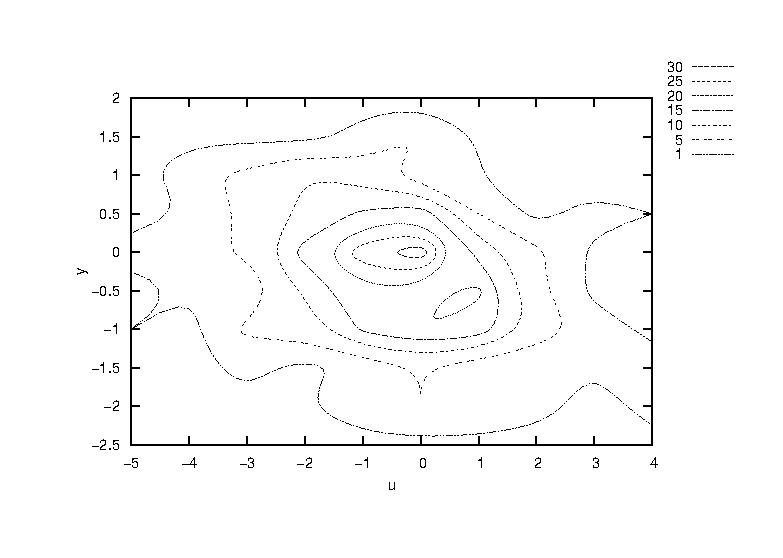
\includegraphics[width=0.8\textwidth,%
  totalheight=0.4\textheight]{u_ny_d2d_ru}
\caption{Двумерное распределение $(u,y)$ с изолиниями равной плотности
  покрытия.}
\label{fig:u_ny_d2d_ru}
\end{figure}

Описанный алгоритм позволяет динамически сформировать обучающее
множество для надежной нейросетевой аппроксимации неизвестной функции,
предсказывающей поведение объекта управления.  Это обучающее множество
используется при настройке НС--О вне контура управления.

\section{Эксперименты}

Оба изложенных подхода --- постоянной адаптации (ПА) и с адаптацией по
обнаружению разладки (АР) --- были реализованы в рамках компьютерной
системы моделирования и нейросетевого управления.  Был проведен ряд
вычислительных экспериментов для изучения свойств и получения
численных оценок качества нейросетевого управления в обоих случаях.
Для оценки качества были взяты два критерия: среднеквадратическая
ошибка управления, дающая представление об интегральных потерях, и
параметры распределения ошибки управления, характеризующие вероятность
пиковых значений ошибки, опасных выходом объекта управления за
технологически допустимые пределы.

\subsection{Стационарные условия}

В серии экспериментов со стационарным объектом управления
исследовалось поведение нейросетевых систем управления в условиях, не
требующих перенастройки.  При использовании нейросетевого регулятора с
постоянной адаптацией наблюдались существенные колебания качества
управления с периодом $2\times 10^5...5\times 10^5$ отчетов и
амплитудой от 0.05 до 6. Это хорошо видно на графике
среднеквадратической ошибки управления
(\figref{fig:steady_plant_errors}).

\begin{figure}[h]
\centering
\includegraphics[width=0.7\textwidth,%
  totalheight=0.3\textheight]{perm_adopt_steady_plant_rus}
\caption{Среднеквадратическая ошибка управления и идентификации в
  стационарных условиях при постоянной адаптации (ПА) и адаптации по
  обнаружению разладки (АР).}
\label{fig:steady_plant_errors}
\end{figure}

Следует отметить, что колебания графика среднеквадратичной ошибки
идентификации $d$ в режиме постоянной адаптации происходили в
противофазе ошибке управления.  Нейросетевой регулятор в рамках
модифицированного подхода обеспечил очень слабые колебания
среднеквадратичной ошибки управления около среднего значения 0.121.
При исследовании статистического распределения ошибки управления было
выявлено, что при адаптации по обнаружению разладки ошибка
распределена по закону, очень близкому к нормальному гауссовскому
(\figref{fig:modif_apr_distrib_rus}).

\begin{figure}[h]
\centering
\includegraphics[width=0.7\textwidth,%
  totalheight=0.3\textheight]{modif_apr_distrib_rus}
\caption{Распределение ошибки управления при адаптации по обнаружению
  разладки в стационарных условиях.}
\label{fig:modif_apr_distrib_rus}
\end{figure}

В режиме постоянной адаптации статистическое распределение ошибки было
непостоянным и в периоды ухудшения качества управления среднее
значение ошибки сильно отличалось от нуля.  Графики распределения
ошибки управления в двух временных интервалах и для всей выборки
приведены на \figref{fig:perm_adopt_distrib_rus}.  Видно, что в
пределах периода хорошего качества управления $[0, 4\times10^5]$
(\figref{fig:steady_plant_errors}) распределение близко к нормальному,
однако в периоды плохого качества управления (например, $[4\times10^5,
  8\times10^5]$) распределение мультимодальное.

\begin{figure}[h]
\centering
\includegraphics[width=0.7\textwidth,%
  height=0.3\textheight]{perm_adopt_distrib_rus}
\caption{Распределение ошибки управления при постоянной адаптации в
  стационарных условиях.}
\label{fig:perm_adopt_distrib_rus}
\end{figure}

Статистические параметры распределения ошибки управления сведены в
\tablref{tabl:steady_state_distrib}.

\begin{table}
  \caption{Параметры распределения ошибки управления в стационарных условиях.}
  \label{tabl:steady_state_distrib}
  \begin{tabular}{|l|c|c|c|c|}
    \hline
    & Минимум & Максимум & Среднее & Дисперсия\\
    \hline
    Постоянная адаптация&
    $-2.03$ & 5.43 & 0.33 & 0.30\\
    \hline
    Адаптация по разладке&
    $-1.46$ & 1.52 & $-0.01$ & 0.12\\
    \hline
  \end{tabular}
\end{table}

\subsection{Изменение параметров объекта управления}

В экспериментах с нестационарным объектом управления его параметры
скачком менялись в момент времени 500.  На
\figref{fig:nonst_cmp_pa_ma_rus} представлены графики
среднеквадратической ошибки при трех разных стратегиях: отсутствие
адаптации нейросетевого регулятора, постоянная адаптация НС--Р и НС--О и
адаптация НС--Р после диагностики разладки, сбора данных и обучения
НС--О вне контура.

\begin{figure}[h]
\centering
\includegraphics[width=0.7\textwidth,%
  height=0.3\textheight]{nonst_cmp_pa_ma_rus}
\caption{Среднеквдратическая ошибка управления в случае разных
  стратегий адаптации.}
\label{fig:nonst_cmp_pa_ma_rus}
\end{figure}

Моменты изменения параметров объекта и начала адаптации нейросетевого
регулятора в рамках подхода с адаптацией по разладке отмечены
вертикальными линиями и подписаны.  Видно, что нейросетевой регулятор
с постоянной адаптацией реагирует на изменение объекта достаточно
быстро и не дает ошибке управления вырасти больше 0.55.  Однако через
некоторое время (примерно $10^4...10^5$) ошибка управления начинает
расти подобно тому, что наблюдалось и при стационарных условиях.

Метод с адаптацией по обнаружению разладки требует сбора данных для
настройки нейросетевого регулятора.  В данном эксперименте объем
выборки для обучения составил 600 отсчетов времени.  За это время
среднеквадратическая ошибка управления успела вырасти до 0.6.  Далее
условно считаем, что настройка нейросетевого идентификатора произошла
мгновенно (это зависит от масштаба времени процесса и доступных
вычислительных мощностей) и в момент времени 1100 началась адаптация
нейросетевого регулятора.  За это время ошибка выросла до 0.7, что
близко к показателю нейросетевого регулятора без адаптации.  После
этого ошибка управления начала планомерно снижаться, причем скорость
снижения была значительно выше, чем в рамках подхода с постоянной
адаптацией.

Статистические параметры ошибки управления в процессе адаптации
приведены в \tablref{tabl:nonst_state_distrib}.

\begin{table}
  \caption{Параметры распределения ошибки управления в нестационарных условиях.}
  \label{tabl:nonst_state_distrib}
  \begin{tabular}{|l|c|c|c|c|}
    \hline
    & Минимум & Максимум & Среднее & Дисперсия\\
    \hline
    Постоянная адаптация&
    $-12.31$ & 3.62 & $-5.23$ & 10.51\\
    \hline
    Адаптация по разладке&
    $-1.98$ & 2.00 & $-0.01$ & 0.46\\
    \hline
  \end{tabular}
\end{table}

\section{Выводы}

\begin{enumerate}
\item Предложены два метода нейросетевого управления нестационарным
  объектом: с постоянной адаптацией и с адаптацией по обнаружению
  разладки.
\item Для обнаружения разладки по дисперсии использовался алгоритм
  кумулятивных сумм.
\item Проведены вычислительные эксперименты с реализацией обоих
  методов на линейном объекте управления.
\item Выявлены свойства обоих рассмотренных подходов нейросетевого
  управления нестационарным объектом.
\item Отмечено большее быстродействие метода управления с постоянной
  адаптацией нейросетевого регулятора по сравнению с методом адаптации
  по обнаружению разладки.
\item Отмечена неустойчивость управления в методе с постоянной
  адаптацией даже в стационарных условиях.
\end{enumerate}
